\subsection{Méthode de tests}
\begin{frame}{Méthode de tests}{Série de tests}
\begin{block}{Complexité}
  \begin{itemize}
    \item Edmonds-Karp : $O(nm^2)$
    \item Dinic : $O(n^2m)$
  \end{itemize}
\end{block}
\begin{block}{Tests effectués}
  \begin{itemize}
    \item Nombre de sommets : 100, 200, 300, \ldots 1000
    \item Densité du graphe : 20\%, 50\% et 80\%
  \end{itemize}
\end{block}
\end{frame}

\begin{frame}{Méthode de tests}{Profiling}
\begin{block}{GNU gprof}
Profiler, analyse du code en fonction du temps passé par chaque fonction à l’exécution.
\begin{itemize}
\item Compilation avec l'argument \texttt{-pg}
\item Exécution du programme, génération du fichier \texttt{gmon.out}
\item Exportation des statistiques en fichier texte
\end{itemize}
\end{block}
\end{frame}

\begin{frame}{Méthode de tests}{Profiling}
\begin{block}{GNU gprof}
Statistique fournies pour chaque fonction :
\begin{itemize}
\item \% temps cpu total
\item temps cpu
\item temps cpu par appel (de manière cumulative ou non)
\end{itemize}
\end{block}
\end{frame}

\subsection{Résultats}
\begin{frame}{Résultats}
\begin{center}
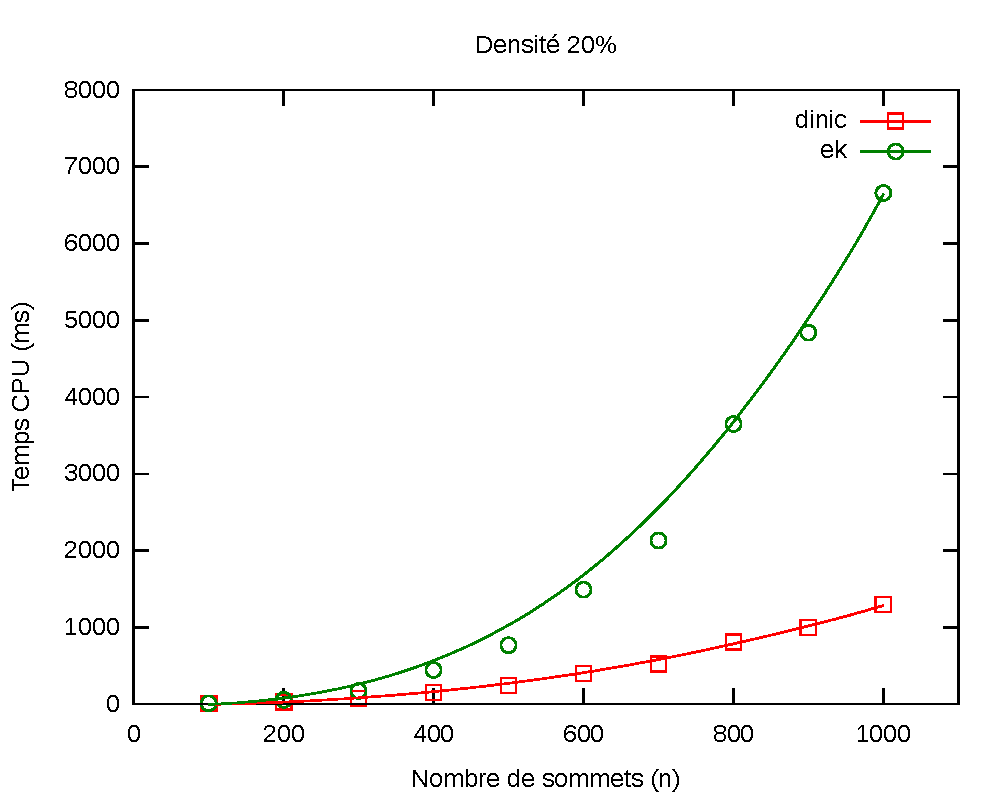
\includegraphics[width=0.8\textwidth]{img/c20}
\end{center}
\end{frame}
\begin{frame}{Résultats}
\begin{center}
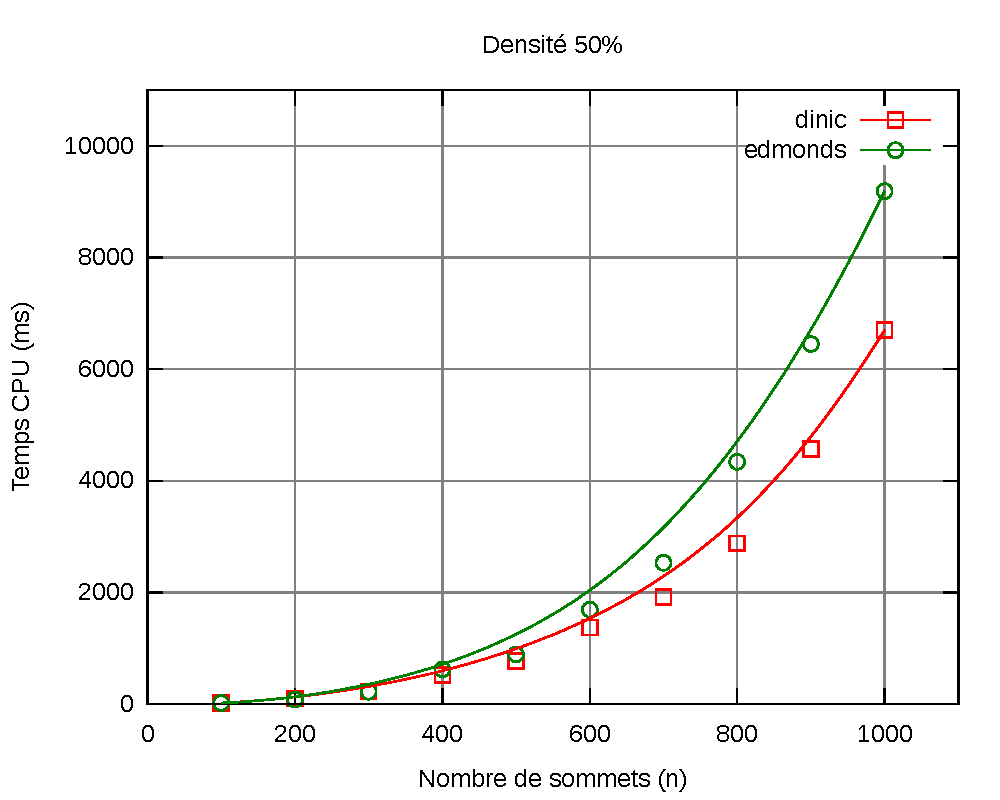
\includegraphics[width=0.8\textwidth]{img/c50}
\end{center}
\end{frame}
\begin{frame}{Résultats}
\begin{center}
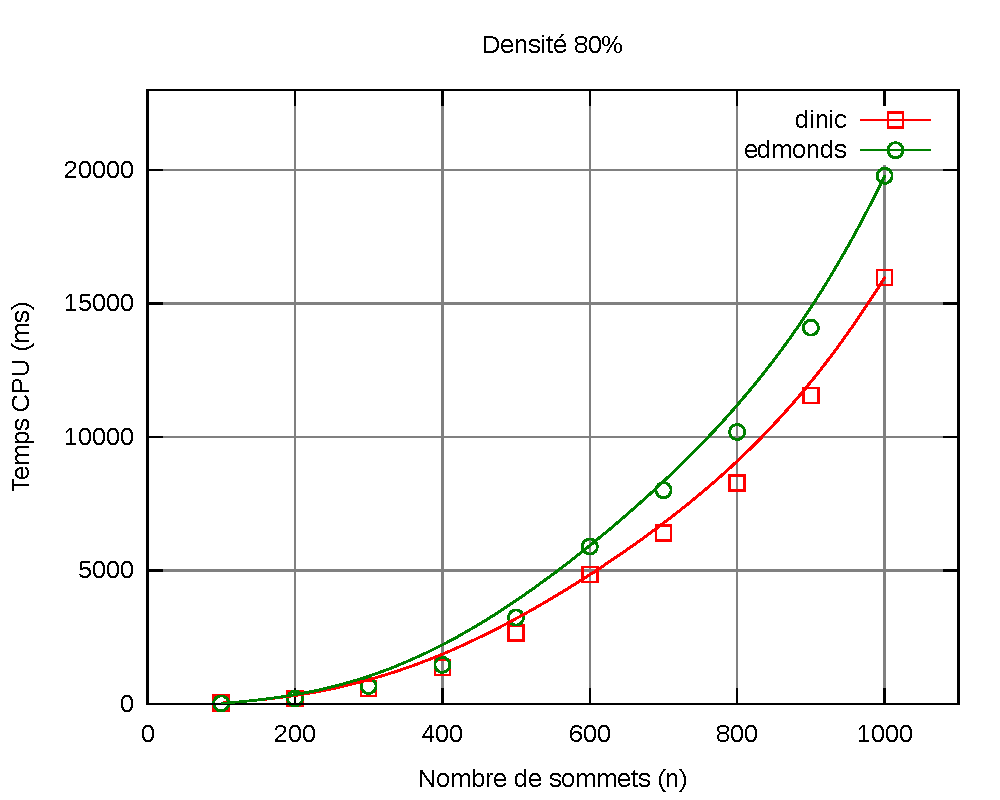
\includegraphics[width=0.8\textwidth]{img/c80}
\end{center}
\end{frame}
\begin{frame}{Résultats}
\begin{center}
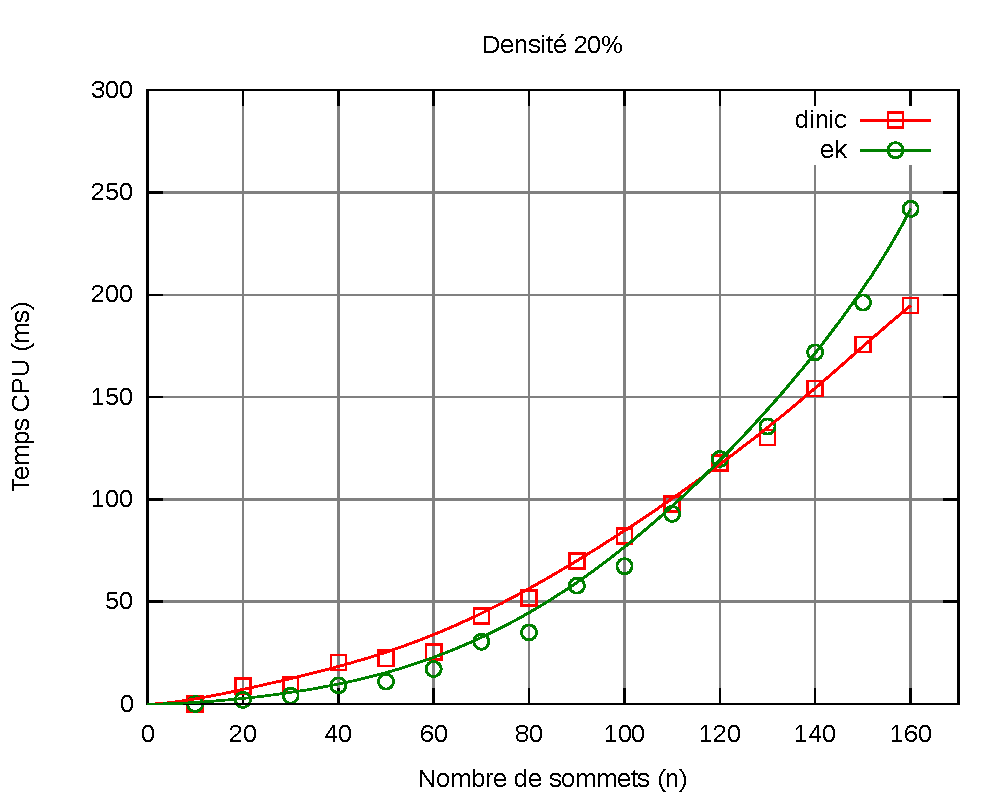
\includegraphics[width=0.8\textwidth]{img/c20_low}
\end{center}
\end{frame}
\begin{frame}{Résultats}
\begin{center}
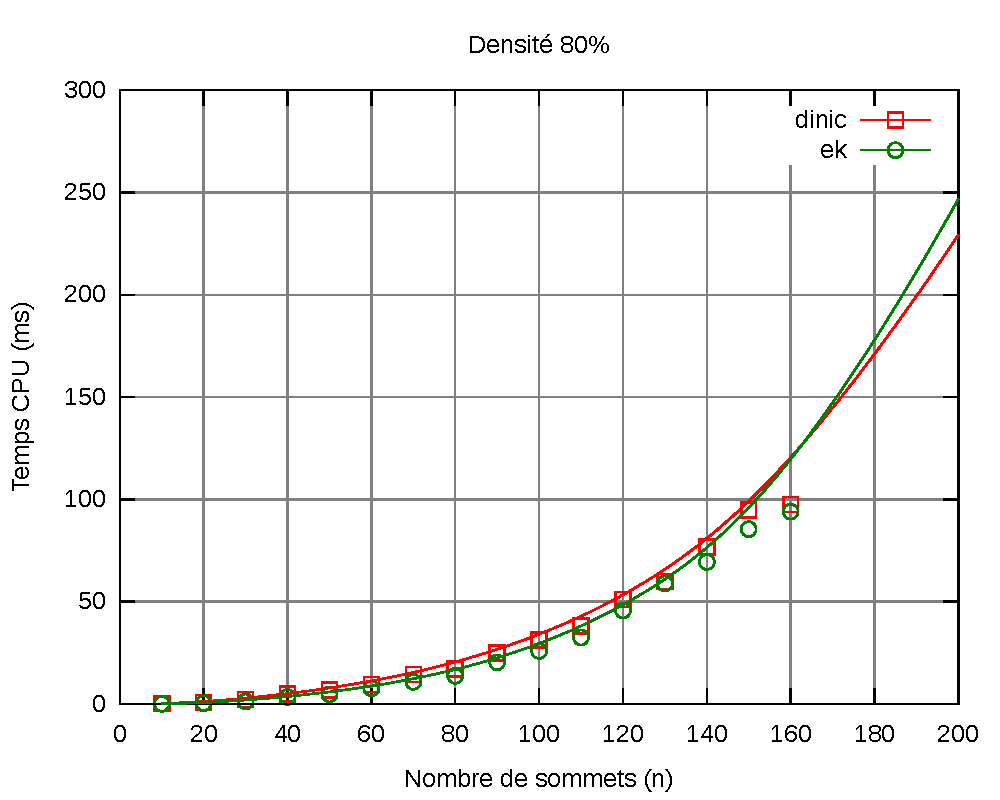
\includegraphics[width=0.8\textwidth]{img/c80_low}
\end{center}
\end{frame}
\begin{frame}{Résultats}{Conclusion}
\begin{itemize}
\item Dinic globalement plus rapide
\item Surtout sur des graphes peu denses
\item Edmonds-Karp efficace sur des petits graphes
\end{itemize}
$\Rightarrow$ Cohérence avec les complexités théoriques
\begin{center}
\begin{tabular}{ccc}
&$\swarrow\ \ \ \ \ \ \searrow$&\\
Dinic&&Edmonds-Karp\\
$O(nm^2)$&&$O(n^2m)$
\end{tabular}
\end{center}
\end{frame}